\section{Проектирование методики обнаружения и архитектуры прототипа}
\label{ch:design}

\noindent
Содержание главы соответствует второму этапу постановки задачи:
проектирование подсистемы предобработки сетевых потоков и схемы
входных представлений модели, архитектуры нейросетевого детектора
со схемой калибровки порога и формирования алертов, архитектуры
конечно-автоматного агента с библиотекой параметризованных шаблонов
трафика и инжектором дрейфа распределений, а также формирование
протокола экспериментального исследования с количественными
критериями принятия.

\subsection{Общая архитектура системы}

Система проектируется в виде четырех подсистем:

\begin{enumerate}
    \item Подсистема предобработки --- валидация схемы потоковых
    данных, нормализация, кодирование, формирование скользящих окон.
    \item Подсистема детекции --- нейросетевая модель, формирующая
    вероятность атаки для каждого окна; калибровка порога.
    \item Подсистема активного тестирования --- программный агент
    на основе конечного автомата с библиотекой шаблонов и
    инжектором дрейфа.
    \item Подсистема алертирования и мониторинга --- формирование
    алертов с уровнями критичности, мониторинг дрейфа распределений,
    дедупликация, экспорт в SOC.
\end{enumerate}

Принципы проектирования: декларативная YAML-конфигурируемость
каждой подсистемы; единый формат представления потокового признака
\texttt{FlowRecord}; слабая связность модулей; совместимость с
RFC 3954 NetFlow v9~\cite{rfc3954} и RFC 7011 IPFIX~\cite{rfc7011}.

Общая архитектура системы и потоки данных между подсистемами
приведены на рисунке~\ref{fig:arch-bpmn}. Синей дорожкой выделена
основная цепочка обнаружения, зелёной --- ветвь мониторинга
дрейфа распределений, оранжевой --- ветвь активного тестирования
FSM-агентом (используется только на стенде).

\begin{figure}[H]
\centering
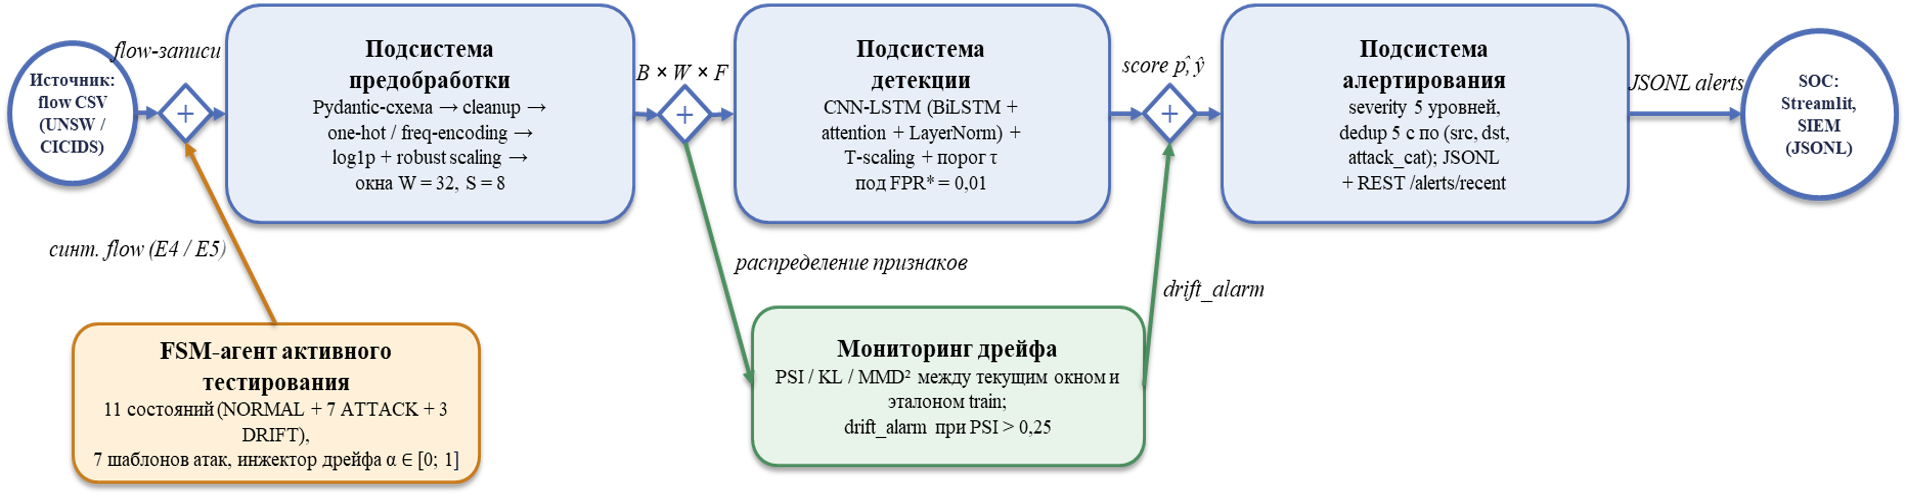
\includegraphics[width=\linewidth]{figures/arch_bpmn.png}
\caption{Общая архитектура методики обнаружения: BPMN-схема
потоков данных с параллельными ветвями мониторинга дрейфа и
активного тестирования}
\label{fig:arch-bpmn}
\end{figure}

Пайплайн обработки одного окна: flow-записи $\to$ схема $\to$
cleanup $\to$ encoding $\to$ scaling $\to$ окно $W \times F$ $\to$
модель $\to$ калибровка $\hat{p}$ $\to$ порог $\tau$ $\to$ алерт
(severity, dedup) $\to$ JSONL / REST.

\subsection{Подсистема предобработки и формирование входных представлений}

\subsubsection{Схема признаков UNSW-NB15}

Датасет UNSW-NB15 содержит 44 содержательных признака, разделяемых
на пять групп (таблица~\ref{tab:unsw-feature-groups})~\cite{moustafa2015unsw,
moustafa2016eval}.

\begin{table}[H]
\caption{Группы признаков UNSW-NB15 и их назначение}
\label{tab:unsw-feature-groups}
\centering
\small
\begin{tabularx}{\linewidth}{|L{2.8cm}|Z|}
\hline
Группа & Состав и роль в детекции \\
\hline
Базовые потоковые &
dur, proto, service, state, sbytes, dbytes, sttl, dttl, sloss,
dloss, rate; длительность, протокол, состояние сессии, байты в обе
стороны, общая скорость потока \\
\hline
Контентные &
sload, dload, swin, dwin, smean, dmean, stcpb, dtcpb, trans\_depth,
response\_body\_len, spkts, dpkts; скорости, окна TCP, базовые
транзакционные характеристики \\
\hline
Временные &
sjit, djit, sinpkt, dinpkt, tcprtt, synack, ackdat; межпакетные
интервалы, джиттеры, RTT, timing-сигнатуры \\
\hline
Дополнительные флаги &
ct\_state\_ttl, ct\_flw\_http\_mthd, is\_ftp\_login, ct\_ftp\_cmd,
is\_sm\_ips\_ports; агрегаты по протокольному поведению, бинарные
флаги \\
\hline
Контекстные ct\_* &
ct\_srv\_src, ct\_srv\_dst, ct\_dst\_ltm, ct\_src\_ltm,
ct\_src\_dport\_ltm, ct\_dst\_sport\_ltm, ct\_dst\_src\_ltm;
агрегаты по последним 100 соединениям; отражают сканирование и
фан-аут \\
\hline
\end{tabularx}
\end{table}

\subsubsection{Pipeline обработки}

Полный pipeline принимает на вход поток flow-записей:
\[
\boxed{
\begin{array}{l}
\text{IPFIX/CSV}\ \to\ \text{Schema}\ \to\ \text{Cleanup}\ \to\ \text{Encoding}\\[2pt]
\to\ \text{Scaling}\ \to\ \text{Windowing}\ \to\ \text{Model}\\[2pt]
\to\ \text{Threshold}\ \to\ \text{Alert}
\end{array}
}
\]

Очистка. Применяются: замена нечисловых пропусков константой,
числовых --- нулем; унификация регистра и пробелов в полях
\texttt{service}, \texttt{state}, \texttt{proto}; удаление
дубликатов; обрезка крайних 0{,}1\,\% хвостов распределений на
основе квантилей 0,001 и 0,999. Вся статистика собирается только
на обучающей выборке, что исключает test-time leakage по
построению.

Кодирование категориальных признаков. One-hot для признаков с
малой кардинальностью (\texttt{proto}, \texttt{state});
frequency-encoding для \texttt{service}:
\begin{equation}
e_{\text{freq}}(c) = \frac{|\{i : x_i^{(c)} = c\}|}{n_{\text{train}}},
\label{eq:freq-enc}
\end{equation}
где \(c\) --- значение категориального признака;
\(n_{\text{train}}\) --- размер обучающей выборки.

Преобразование числовых признаков. Лог-преобразование
тяжелохвостых признаков \(\tilde{x} = \log(1 + x)\) с последующим
robust-scaling:
\begin{equation}
\tilde{x}' = \frac{\tilde{x} - \operatorname{med}(\tilde{x})}
                  {\operatorname{IQR}(\tilde{x})},
\label{eq:robust-scaler}
\end{equation}
где \(\operatorname{med}\) --- медиана признака по обучающей
выборке; \(\operatorname{IQR}\) --- межквартильный размах.
Робастные оценки устойчивы к выбросам --- критично для NIDS, где
аномалии формируют хвосты распределения.

Скользящие окна. Принят размер \(W = 32\) с шагом \(S = 8\)
(75\,\% перекрытие). Метка окна формируется по последнему flow
(last-агрегация) с учетом эмпирически обоснованной структуры
UNSW-NB15.

\subsubsection{Управление дисбалансом классов}

Применяется focal loss~\cite{lin2017focal}:
\begin{equation}
\mathcal{L}_{\text{focal}} =
-\frac{1}{n}\sum_{i=1}^{n}
  \alpha_{y_i}\,(1-p_{y_i})^{\gamma}\,\log p_{y_i},
\label{eq:focal}
\end{equation}
где \(p_{y_i}\) --- предсказанная вероятность истинного класса для
\(i\)-го объекта; \(\alpha_{y_i}\) --- весовой коэффициент класса
(\(\alpha = 0{,}25\) для положительного класса);
\(\gamma\) --- параметр фокусирования (\(\gamma = 2{,}0\)).
Для классических baselines дополнительно применяется class
re-weighting \(w_c = n / (|\mathcal{C}|\,n_c)\).

\subsection{Архитектура нейросетевого детектора}

\subsubsection{Целевая архитектура CNN-LSTM}

По результатам балльной оценки этапа~\ref{ch:theory} в качестве
целевой архитектуры принят гибрид CNN-LSTM. Детальная схема:
\begin{equation*}
\begin{aligned}
\text{Input}(B, W, F)\ &\to\ \underbrace{[\text{Conv1D}\!\to\!\text{BN}\!\to\!\text{ReLU}\!\to\!\text{MaxPool}\!\to\!\text{Dropout}]\!\times\!2}_{\text{два сверточных блока}}\\
&\to\ \text{BiLSTM}\ \to\ \text{Attention\,Pool}\ \to\ \text{LayerNorm}\ \to\ \text{MLP-head}\ \\ \to\ \text{Sigmoid}.
\end{aligned}
\end{equation*}

Усиления относительно базовой схемы CNN-LSTM:
двунаправленный LSTM по умолчанию (стандартная практика NIDS-публикаций
2024--2025~\cite{ahmad2021nids, vinayakumar2019dl});
attention-пулинг над выходами LSTM вместо последнего скрытого
состояния, стабилизирующий обучение по seed;
LayerNorm перед head, снимающий scale drift между Conv и LSTM
активациями.

Полная блочная диаграмма детектора с указанием размерностей
тензоров и гиперпараметров каждого слоя, а также схемой
постпроцессинга (температурная калибровка, поиск порога
$\tau$ под целевой FPR, бинарное решение, severity-классификация)
приведена на рисунке~\ref{fig:arch-cnn-lstm}.

\begin{figure}[H]
\centering
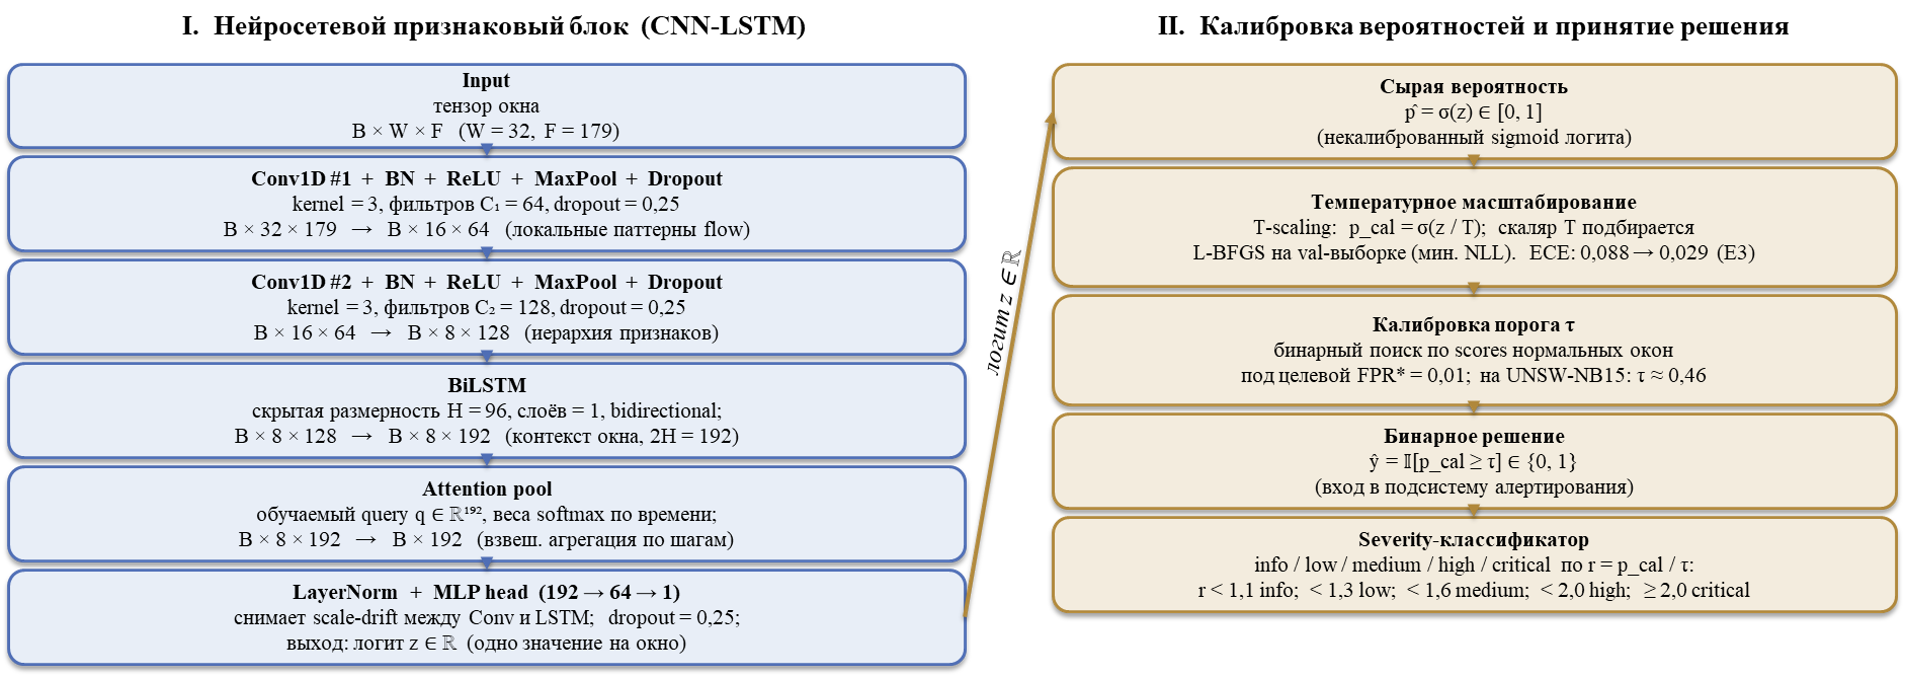
\includegraphics[width=\linewidth]{figures/arch_cnn_lstm.png}
\caption{Двухдорожечная блочная диаграмма детектора CNN-LSTM:
дорожка I --- извлечение признаков нейросетью; дорожка II ---
калибровка вероятностей и принятие решения}
\label{fig:arch-cnn-lstm}
\end{figure}

\subsubsection{Совокупность альтернативных моделей}

Для эксперимента в равных условиях реализуются 15 моделей-кандидатов
в едином программном регистре. Состав регистра приведен в
таблице~\ref{tab:models-impl}.

\begin{table}[H]
\caption{Совокупность моделей-кандидатов в едином регистре}
\label{tab:models-impl}
\centering
\small
\begin{tabularx}{\linewidth}{|L{2.3cm}|L{2.8cm}|Z|}
\hline
Имя & Тип & Назначение \\
\hline
mlp                  & DL supervised & нижняя граница DL-семейства \\
\hline
cnn1d                & DL supervised & базовая сверточная сеть \\
\hline
cnn\_lstm            & DL supervised, proposed & целевая архитектура \\
\hline
lstm                 & DL supervised & рекуррентный baseline \\
\hline
gru                  & DL supervised & облегченная RNN \\
\hline
bilstm               & DL supervised, attn & двунаправленный контекст \\
\hline
tcn                  & DL supervised & темпоральные дилатир. свертки \\
\hline
transformer          & DL supervised & self-attention encoder \\
\hline
autoencoder          & DL semi-supervised & semi-supervised режим \\
\hline
vae                  & DL semi-supervised & вариационный AE \\
\hline
\makecell[l]{logistic\_\\ regression} & classical & линейный baseline \\
\hline
\makecell[l]{random\_\\ forest}       & classical & ансамблевый baseline \\
\hline
xgboost              & classical & gradient boosting baseline \\
\hline
\makecell[l]{isolation\_\\ forest}    & classical unsup. & unsupervised \\
\hline
ocsvm                & classical one-class & one-class режим \\
\hline
\end{tabularx}
\end{table}

\subsubsection{Сценарий обучения}

Гиперпараметры обучения зафиксированы в таблице~\ref{tab:train-hyperparams}.

\begin{table}[H]
\caption{Гиперпараметры обучения DL-моделей}
\label{tab:train-hyperparams}
\centering
\begin{tabularx}{\linewidth}{|L{4.0cm}|L{3.0cm}|Z|}
\hline
Параметр & Значение & Назначение \\
\hline
Оптимизатор          & AdamW                 & адаптивный градиентный метод \\
\hline
Learning rate        & $1{,}0 \cdot 10^{-3}$ & базовая скорость обучения \\
\hline
Weight decay         & $1{,}0 \cdot 10^{-4}$ & регуляризация \\
\hline
Batch size           & 256                   & размер минибатча \\
\hline
Эпохи (макс.)        & 30 (60 для CNN-LSTM)  & лимит обучения \\
\hline
Patience             & 7 (12 для CNN-LSTM)   & окно early stopping \\
\hline
Метрика мониторинга  & val\_pr\_auc          & метрика остановки \\
\hline
LR-scheduler         & cosine annealing      & снижение lr к $10^{-6}$ \\
\hline
Gradient clipping    & $\|g\|_2 \leq 1{,}0$  & защита от взрыва градиентов \\
\hline
Loss-функция         & focal loss            & противодействие дисбалансу \\
\hline
$\alpha$ (focal)     & $0{,}25$              & вес положительного класса \\
\hline
$\gamma$ (focal)     & $2{,}0$               & фокусировка на трудных примерах \\
\hline
Seed                 & 42, 123, 2024         & 3 запуска для proposed \\
\hline
\end{tabularx}
\end{table}

\subsection{Калибровка вероятностей и порога принятия решения}

Применяется однопараметрическое температурное
масштабирование~\cite{guo2017calibration} логитов на валидационной
выборке через L-BFGS, минимизирующее
negative log-likelihood. Затем выполняется поиск порога $\tau^*$
под целевую частоту ложных срабатываний $\operatorname{FPR}^* = 0{,}01$
бинарным поиском по отсортированному списку скорингов нормальных
окон. Качество калибровки оценивается по Expected Calibration Error
с 15 биннами равной ширины.

\subsection{Подсистема алертирования}

Принимается пятиступенчатая шкала severity, согласованная с
типовыми классификациями SIEM:

\begin{table}[H]
\caption{Шкала уровней критичности алертов}
\label{tab:severity-ladder}
\centering
\begin{tabularx}{\linewidth}{|L{2.0cm}|L{3.5cm}|Z|}
\hline
Уровень & Условие $s / \tau$ & Действие SOC \\
\hline
info & $[1{,}0;\, 1{,}1)$ & информационное событие \\
\hline
low & $[1{,}1;\, 1{,}3)$ & стандартный обзор L1 \\
\hline
medium & $[1{,}3;\, 1{,}6)$ & приоритетный обзор, передача L2 \\
\hline
high & $[1{,}6;\, 2{,}0)$ & передача L2, расследование \\
\hline
critical & $\geq 2{,}0$ & немедленное расследование \\
\hline
\end{tabularx}
\end{table}

Дополнительно реализуется временная дедупликация алертов с
$\Delta t_{\text{dedup}} = 5$~с по триплету (src\_ip, dst\_ip,
attack\_cat) для подавления шумовых повторов одного инцидента.

\subsection{Архитектура конечно-автоматного агента активного тестирования}

\subsubsection{Состояния и политика}

Принимается 11 состояний конечного автомата:
\[
\mathcal{S} = \{\text{NORMAL}\} \cup \{\text{ATTACK}(c)\}_{c \in \mathcal{C}}
\cup \{\text{DRIFT}(k)\}_{k \in \mathcal{K}},
\]
где $\mathcal{C} = \{\text{DDoS, Scan, Brute, Exploit, Exfil, IntRec, Worm}\}$,
$\mathcal{K} = \{\text{covariate, prior, concept}\}$. Политика
$\pi : \mathcal{S} \to \Delta(\mathcal{S})$ задается стохастической
матрицей вероятностей переходов в YAML-конфигурации с
минимальными длительностями состояний.

\subsubsection{Библиотека шаблонов атак}

Реализуются семь параметризованных шаблонов атак плюс шаблон
\texttt{normal} (таблица~\ref{tab:attack-templates}).

\begin{table}[H]
\caption{Реализованная библиотека шаблонов атак}
\label{tab:attack-templates}
\centering
\small
\begin{tabularx}{\linewidth}{|L{2.4cm}|Z|L{2.8cm}|}
\hline
Шаблон & Параметризация & Класс UNSW \\
\hline
\makecell[l]{ddos\_\\ synflood} &
интенсивность $\lambda_0$, длительность, доля SYN, распределение
исходных IP &
DoS \\
\hline
\makecell[l]{port\_\\ scan} &
скорость подключений $\rho$, диапазон портов, режим, длительность &
Reconnaissance \\
\hline
\makecell[l]{brute\_\\ force} &
интервал между попытками, целевой порт, доля успехов &
Reconnaissance / Exploits \\
\hline
\makecell[l]{exploit\_\\ payload} &
размер payload, сочетания TCP-флагов, доля retransmissions &
Exploits \\
\hline
\makecell[l]{data\_\\ exfil} &
длительность сессии, асимметрия $b_{out}/b_{in}$, стабильность
скорости &
Backdoors \\
\hline
\makecell[l]{internal\_\\ recon} &
фан-аут потоков, периодичность, размер сессии &
Reconnaissance \\
\hline
\makecell[l]{worm\_\\ lateral} &
число направленных потоков, периодичность, размер сессии &
Worms \\
\hline
\end{tabularx}
\end{table}

Шаблоны реализуются в двух режимах:
эмпирическом (фитятся на выборке UNSW-NB15-train, sampling из
эмпирических распределений по \texttt{attack\_cat}) и
параметрическом (вручную параметризованные диапазоны, fallback).
Эмпирический режим обеспечивает близость к маргинальным
распределениям источника и используется в production-режиме.

\subsubsection{Инжектор дрейфа распределений}

Реализуются три типа дрейфа согласно типологии Gama и
соавт.~\cite{gama2014drift}.

Covariate drift. Изменение $P(X)$ при фиксированном $P(Y \mid X)$:
\[
x'_i = (1 + \alpha \cdot u_i) \cdot x_i + \alpha \cdot \sigma_i \cdot \varepsilon_i,
\]
где $u_i \sim \mathcal{U}(-0{,}5; 0{,}5)$, $\varepsilon_i \sim
\mathcal{N}(0, 1)$, $\sigma_i$ --- стандартное отклонение признака
на train, $\alpha$ --- интенсивность дрейфа.

Prior drift. Изменение $P(Y)$ при сохранении $P(X \mid Y)$ через
изменение долей классов в политике FSM.

Concept drift. Изменение $P(Y \mid X)$ через маскирование
сигнатурных признаков атак (зануление или подмена характерных
значений \texttt{state}, ct\_*-агрегатов).

Контроль интенсивности --- параметр $\alpha \in \{0; 0{,}25; 0{,}5;
0{,}75; 1{,}0\}$.

\subsection{Подсистема мониторинга дрейфа}

Реализуются три индекса, взаимно дополняющих друг друга. PSI ---
по маржинальным распределениям, с устоявшимся в практике порогом
$\operatorname{PSI} > 0{,}25$; KL-расхождение по биннам;
$\operatorname{MMD}^2$ с гауссовым ядром и автобандвидтом по
медианной эвристике. Подсистема возвращает агрегированный отчет
\texttt{drift\_report} с индикатором \texttt{drift\_alarm}.

\subsection{Протокол экспериментального исследования}

Сформирован протокол шести экспериментов (таблица~\ref{tab:experiments})
плюс cross-evaluation и демонстрационный прогон в реальном
времени.

\begin{table}[H]
\caption{Протокол экспериментального исследования}
\label{tab:experiments}
\centering
\small
\setlength{\tabcolsep}{4pt}
\begin{tabularx}{\linewidth}{|c|Z|Z|Z|}
\hline
ID & Цель & Метрики & Критерий принятия \\
\hline
E1 &
Сравнение 15 моделей в равных условиях на UNSW-NB15 &
Precision, Recall, F1, MCC, PR-AUC, ROC-AUC, $\sigma_{F1}$ &
F1 ≥ 0,90; PR-AUC ≥ 0,95; ${p}\,{<}\,0{,}05$ vs ансамбль baselines \\
\hline
E2 &
Анализ ошибок CNN-LSTM по \texttt{attack\_cat} &
confusion matrix, per-class recall &
идентификация классов с пониженной полнотой \\
\hline
E3 &
Калибровка порога; температурное масштабирование &
ECE до/после, $T^*$, $\tau^*$, FPR на test &
ΔECE ≥ 30\,\% для CNN-LSTM \\
\hline
E4 &
Стресс-тест с FSM-агентом, per-state recall &
F1, Precision, Recall, per-state recall, FPR &
per-state recall ≥ 0{,}50 для ≥ 5 классов \\
\hline
E5 &
Drift-устойчивость; PSI/MMD-инжектирование &
F1, PR-AUC vs $\alpha$; PSI, MMD; drift\_alarm &
ΔF1 ≤ 0,10 при PSI ≤ 0,25; drift\_alarm срабатывает при PSI > 0,25 \\
\hline
E6 &
Эксплуатационная производительность &
inference latency, throughput, CPU/RAM &
NFR-3 (≤ 50 мс), NFR-4 (≥ 1000 EPS) \\
\hline
\end{tabularx}
\end{table}

Для каждого эксперимента применяются: множественные seed
(\(n \geq 3\) для лидирующих моделей), bootstrap CI 95\,\%, парный
критерий Уилкоксона при сравнении пар моделей, фиксированные
YAML-конфиги.

\noindent Выводы по главе 2

\begin{enumerate}
    \item Спроектирована четырехподсистемная архитектура с
    декларативной YAML-конфигурируемостью и совместимостью с
    NetFlow v9 / IPFIX.
    \item Описана теоретическая модель данных и pipeline обработки
    UNSW-NB15: схема признаков, очистка, encoding, log-преобразование,
    robust-scaling, скользящие окна $W=32$, $S=8$, last-агрегация
    меток, focal loss для управления дисбалансом классов.
    \item Зафиксирована детальная схема целевой архитектуры
    CNN-LSTM с двунаправленным LSTM, attention-пулингом и
    LayerNorm; реализован регистр из 15 моделей-кандидатов.
    \item Спроектирована двухступенчатая калибровка: температурное
    масштабирование + поиск порога под target-FPR; пятиступенчатая
    шкала severity и временная дедупликация.
    \item Сформирована архитектура конечно-автоматного агента с
    11 состояниями, 7 шаблонами атак, инжектором дрейфа трех типов
    в эмпирическом и параметрическом режимах.
    \item Сформирован протокол шести экспериментов E1--E6 с
    количественными критериями принятия.
\end{enumerate}
